\documentclass[../Main.tex]{subfiles}

\begin{document}
\author{Stationary Waves} %use author for title of lesson
\date{Year 1 Topic 19} %use date to refer to topic in main booklet

\section{Stationary Waves} %Section is the title of the lesson repeated, ready for the main contents page.

\begin{frame}{Reflected Waves}
    Imagine a progressive wave that reflects off a surface back to the source, while the original wave continues emitting. Since the wave and its reflection are both travelling, there will be points where they always reach each other exactly in phase, and points where they reach each other exactly antiphase \newline 
    
    \newline-- note that this does not necessarily have to be a reflection, it just has to be the same amplitude and frequency!
    \begin{figure}
        \centering
        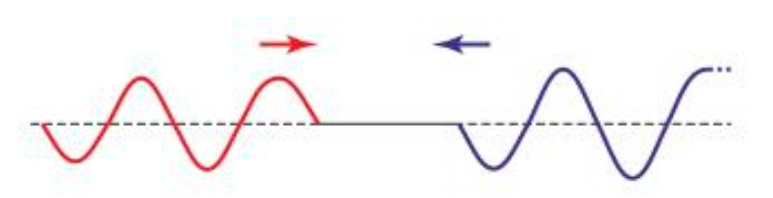
\includegraphics[height=2cm]{Waves_Images/incomingwaves.jpg}
    \end{figure}
    
\end{frame}

\begin{frame}{Stationary Waves}
    The resulting superposition of the waves has regions of no amplitude (called nodes) and points of maximum amplitude (antinodes) -- we call these stationary waves.
    
    \begin{figure}
        \centering
        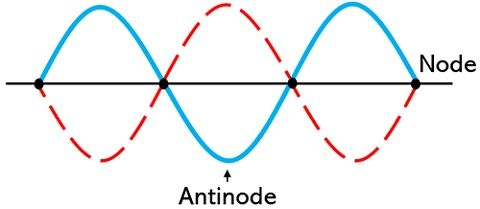
\includegraphics[width=0.6\textwidth]{Waves_Images/stationary-wave.jpg}
    \end{figure}
    We call these stationary waves because the resulting wave does not progress -- a displacement-distance graph would not change with time, save for an oscillation, hence the dashed line. \newline
    \newline
    -- Simulation: \url{https://ophysics.com/w8.html}
\end{frame}

\begin{frame}{Properties of Stationary Waves}
\begin{itemize}
    \item On a stationary wave, the distance between two adjacent antinodes (or two adjacent nodes) is half the wavelength of the original waves.
    \item There is no overall propagation of energy -- all energy is ``stuck" at the antinodes -- more on this soon!
\end{itemize}
\begin{figure}
    \centering
    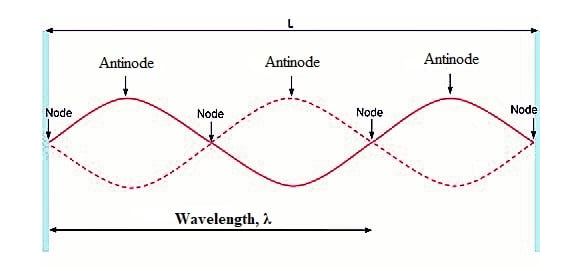
\includegraphics[width=9cm]{Waves_Images/Stationary-wave.png}
\end{figure}
\end{frame}

\begin{frame}{Examples}
    \begin{exampleblock}{Example 1}
    \begin{figure}
        \centering
        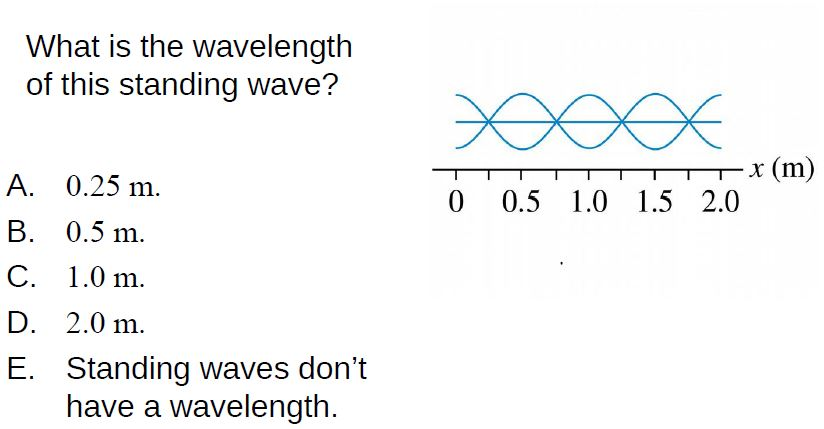
\includegraphics[height=3cm]{Waves_Images/stationarywave_mcq.jpg}
    \end{figure}
    \end{exampleblock}
\end{frame}

\begin{frame}{Progressive vs Stationary Waves}
Let's compare progressive to stationary waves...
\tiny
\begin{table}[]
\begin{tabular}{l|l|l}
 & Progressive Wave & Stationary Wave \\ \hline
energy transfer  & \begin{tabular}[c]{@{}l@{}}is either parallel or perpendicular\\  to the oscillation of the wave\end{tabular}  & no net energy transfer \\ \hline
wavelength  & \begin{tabular}[c]{@{}l@{}}the distance between two points \\ that are in phase in adjacent cycles\end{tabular}  & \begin{tabular}[c]{@{}l@{}}double the distance between two \\ adjacent nodes (or antinodes)\end{tabular} \\ \hline
phase difference  & \begin{tabular}[c]{@{}l@{}}is different between any two points \\ on the wave\end{tabular}  & \begin{tabular}[c]{@{}l@{}}is constant for any two points on \\ the wave (0 rad or $\pi$ rad.)\end{tabular} \\ \hline
amplitude  & \begin{tabular}[c]{@{}l@{}}each point of the wave has the same \\ amplitude  but at a different phase\end{tabular}  & \begin{tabular}[c]{@{}l@{}}is different anywhere on the wave, \\ but maximum at antinodes.\end{tabular}
\end{tabular}
\end{table}
\end{frame}

\end{document}